\startchapter{Results and Discussion}
\label{chapter:eval}
\section{Results} \label{sec:Results}
\subsection{Methodology}
\acrlong{IC} manufacturers distribute their product to devices which control everything from cell phones to fighter jets. 
Those who employ \acrlong{FPGAs} require the means to ensure that their chips function as intended. 
The \NameNoPeriod provides manufacturers a quick means of ensuring that they are providing a safe and secure product to their customers.
To demonstrate its potential, it has been tested using a series of benchmarks.
These benchmarks are included in the \NameNoPeriod application package as an example for users.
\subsection{Priority Decoder} \label{sec:priorityDecoder}
At the \acrfull{ISCAS} in 1989, F. Brglez and H. Fujiwara presented a series of \acrshort{FPGA} benchmark circuits originally written in C~\cite{iscas85}. 
These benchmarks were accessed and a small 'Priority Decoder' circuit was chosen~\cite{iscasBenchmarks}.
The provided verilog code for the decoder benchmark was synthesized on a Virtex-5 XC5VLX155 and the generated \gls{Bitstream} and \acrshort{XDL} files were acquired.
The priority decoder \gls{Bitstream} file was fed to both the \gls{golden} and \gls{target} inputs to the \Name.
Feeding the same \gls{Bitstream} file to both inputs replicates the occurrence where the third-party fabrication house made no modifications; the \gls{Bitstream} extracted from the \gls{target} device is exactly the same as the \gls{golden}.
It is expected that the \NameNoPeriod returns a result indicating that there is no trojan present.
As can be seen in Figure~\ref{fig:priorityDecoder}, the \NameNoPeriod successfully analyzed the \gls{Bitstream}s and determined that there was no trojan present, as expected.
\begin{figure}
\centering
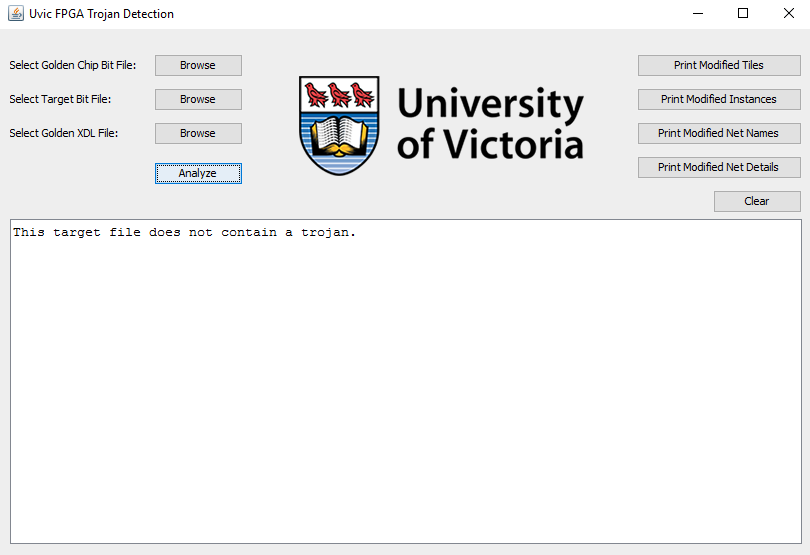
\includegraphics[width=1\linewidth]{Figures/priorityDecoder}
\caption[Priority Decoder Analysis Results]{Priority Decoder Analysis Results}
\label{fig:priorityDecoder}
\end{figure}

\subsection{User Authentication Circuit} \label{sec:userAuthentication}
Consider a circuit designed to compute a function $F(x)$ for a system to authenticate user-password pairs $x$ and $F(x)$.
The system performs the arithmetic operation $F(x) = x^2$ to validate users.
The customer wishes to provide access to ten users labeled $I_0$ to $I_9$.
To identify all ten users, four input bits are required, $x_1$ to $x_4$.
The largest function output is $81$ meaning seven bits are required for output, $Z_1$ to $Z_7$, as illustrated in Fig.~\ref{fig:userAuthenticationCircuit}.
\begin{figure*}[h]
	\centering
	\begin{subfigure}[t]{0.5\textwidth}
		\centering
		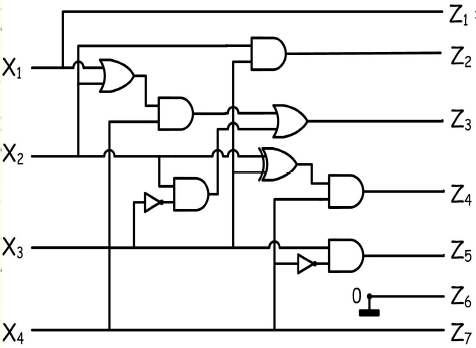
\includegraphics[height=2in]{Figures/circuit1}
		\caption{A Simple User Authentication Circuit}
		\label{fig:userAuthenticationCircuit}
	\end{subfigure}%
	~ 
	\begin{subfigure}[t]{0.5\textwidth}
		\centering
		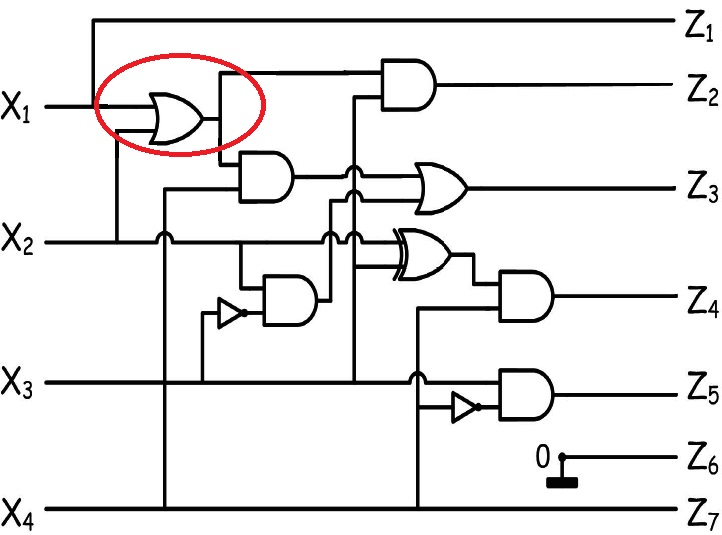
\includegraphics[height=2in]{Figures/circuit2}
		\caption{The Back-door Trojan}
		\label{fig:userAuthenticationCircuitTrojan}
	\end{subfigure}
	\caption{The User Authentication Circuit: Clean and Trojan}
	\label{fig:userAuthentication}
\end{figure*}
\begin{table*}[]
	\setlength{\tabcolsep}{3pt}
	\centering
	\caption{Outputs of the Circuits in Figs.~\ref{fig:userAuthenticationCircuit} and \ref{fig:userAuthenticationCircuitTrojan}~\cite{samerAttribute}}
	\label{tbl:trojanOutputs}
	\begin{tabular}{CC|C|C|C|C|C||C|C|C|C|C|C|C|C||C|C|C|C|C|C|C|C|}
		\cline{3-23}
		&  & \multicolumn{5}{c||}{Inputs} & \multicolumn{8}{c||}{Circuit A} & \multicolumn{8}{c|}{Circuit B} \\ \cline{3-23}
		&  & X_1 & X_2 & X_3 & X_4 & X & Z_1 & Z_2 & Z_3 & Z_4 & Z_5 & Z_6 & Z_7 & F(x) & Z_1 & Z_2 & Z_3 & Z_4 & Z_5 & Z_6 & Z_7 & F(x) \\ \hline
		\multicolumn{1}{|c|}{\multirow{10}{*}{\rotatebox[origin=c]{90}{Inputs}}} & I_0 & 0 & 0 & 0 & 0 & 0 & 0 & 0 & 0 & 0 & 0 & 0 & 0 & 0 & 0 & 0 & 0 & 0 & 0 & 0 & 0 & 0 \\ \cline{2-23}
		\multicolumn{1}{|c|}{} & I_1 & 0 & 0 & 0 & 1 & 1 & 0 & 0 & 0 & 0 & 0 & 0 & 1 & 1 & 0 & 0 & 0 & 0 & 0 & 0 & 1 & 1 \\ \cline{2-23}
		\multicolumn{1}{|c|}{} & I_2 & 0 & 0 & 1 & 0 & 2 & 0 & 0 & 0 & 0 & 1 & 0 & 0 & 4 & 0 & 0 & 0 & 0 & 1 & 0 & 0 & 4 \\ \cline{2-23}
		\multicolumn{1}{|c|}{} & I_3 & 0 & 0 & 1 & 1 & 3 & 0 & 0 & 0 & 1 & 0 & 0 & 1 & 9 & 0 & 0 & 0 & 1 & 0 & 0 & 1 & 9 \\ \cline{2-23}
		\multicolumn{1}{|c|}{} & I_4 & 0 & 1 & 0 & 0 & 4 & 0 & 0 & 1 & 0 & 0 & 0 & 0 & 16 & 0 & 0 & 1 & 0 & 0 & 0 & 0 & 16 \\ \cline{2-23}
		\multicolumn{1}{|c|}{} & I_5 & 0 & 1 & 0 & 1 & 5 & 0 & 0 & 1 & 1 & 0 & 0 & 1 & 25 & 0 & 0 & 1 & 1 & 0 & 0 & 1 & 25 \\ \cline{2-23}
		\multicolumn{1}{|c|}{} & I_6 & 0 & 1 & 1 & 0 & 6 & 0 & 1 & 0 & 0 & 1 & 0 & 0 & 36 & 0 & 1 & 0 & 0 & 1 & 0 & 0 & 36 \\ \cline{2-23}
		\multicolumn{1}{|c|}{} & I_7 & 0 & 1 & 1 & 1 & 7 & 0 & 1 & 1 & 0 & 0 & 0 & 1 & 49 & 0 & 1 & 1 & 0 & 0 & 0 & 1 & 49 \\ \cline{2-23}
		\multicolumn{1}{|c|}{} & I_8 & 1 & 0 & 0 & 0 & 8 & 1 & 0 & 0 & 0 & 0 & 0 & 0 & 64 & 1 & 0 & 0 & 0 & 0 & 0 & 0 & 64 \\ \cline{2-23}
		\multicolumn{1}{|c|}{} & I_9 & 1 & 0 & 0 & 1 & 9 & 1 & 0 & 1 & 0 & 0 & 0 & 1 & 81 & 1 & 0 & 1 & 0 & 0 & 0 & 1 & 81 \\ \hline
		\multicolumn{1}{|c|}{\multirow{6}{*}{\rotatebox[origin=c]{90}{Undefined}}} & I_{10} & 1 & 0 & 1 & 0 & 10 & 1 & 0 & 0 & 0 & 1 & 0 & 0 & 68 & 1 & 1 & 0 & 0 & 1 & 0 & 0 & 100 \\ \cline{2-23}
		\multicolumn{1}{|c|}{} & I_{11} & 1 & 0 & 1 & 1 & 11 & 1 & 0 & 1 & 1 & 0 & 0 & 1 & 89 & 1 & 1 & 1 & 1 & 0 & 0 & 1 & 121 \\ \cline{2-23}
		\multicolumn{1}{|c|}{} & I_{12} & 1 & 1 & 0 & 0 & 12 & 1 & 1 & 1 & 0 & 0 & 0 & 0 & 112 & 1 & 0 & 1 & 0 & 0 & 0 & 0 & 80 \\ \cline{2-23}
		\multicolumn{1}{|c|}{} & I_{13} & 1 & 1 & 0 & 1 & 13 & 1 & 1 & 1 & 1 & 0 & 0 & 1 & 121 & 1 & 0 & 1 & 1 & 0 & 0 & 1 & 89 \\ \cline{2-23}
		\multicolumn{1}{|c|}{} & I_{14} & 1 & 1 & 1 & 0 & 14 & 1 & 1 & 0 & 0 & 1 & 0 & 0 & 100 & 1 & 1 & 0 & 0 & 1 & 0 & 0 & 100 \\ \cline{2-23}
		\multicolumn{1}{|c|}{} & I_{15} & 1 & 1 & 1 & 1 & 15 & 1 & 1 & 1 & 0 & 0 & 0 & 1 & 113 & 1 & 1 & 1 & 0 & 0 & 0 & 1 & 113 \\ \hline
	\end{tabular}
\end{table*}
A trojan can be inserted into this circuit as shown in Fig.~\ref{fig:userAuthenticationCircuitTrojan} (called a backdoor trojan).
The outputs of the original and infected circuits are compared in Table~\ref{tbl:trojanOutputs}.
A simple test will show that the circuit outputs the desired $F(x) = x^2$ for each of the users.
However, upon closer inspection it is noted that the inputs corresponding to $x = 10$ to $x = 15$ are not used; there are no clients occupying those identifications.
These unused inputs are referred to as 'dont-cares', meaning that it is not important to the function of the circuit what their corresponding output is.
Don't-care cases are a typical vulnerability which can be exploited by an attacker.
Under the 'Circuit A' column of Table~\ref{tbl:trojanOutputs} it can be seen that $I_{10}$ and $I_{11}$ produce results 68 and 89 respectively.
These results are not correct according to $F(x) = x^2$.
This is an intended result by the circuit designer to add security for these don't care conditions.
If an attacker is able to make the modification in Fig.~\ref{fig:userAuthenticationCircuitTrojan}, inputs $10$ and $11$ will now produce results 100 and 121 which are correct according to $F(x) = x^2$.
This can be seen under the 'Circuit B' column of Table~\ref{tbl:trojanOutputs}.
Now, the attacker has built a 'back-door' into the circuit.
The original 10 users' authentication is not altered but inputs 10 and 11 provide unauthorized access to the attacker.

The circuits shown in Figure~\ref{fig:userAuthentication} were implemented using \Xilinx's schematic designer and placed on a Virtex-5 240T (XC5VSX240T).
The \gls{Bitstream}s and \acrshort{XDL} files were generated and input to the \Name.
The analysis detected a trojan and output the list of determined attributes as can be seen in Figure~\ref{fig:backDoorResult}.
\begin{figure}[h]
\centering
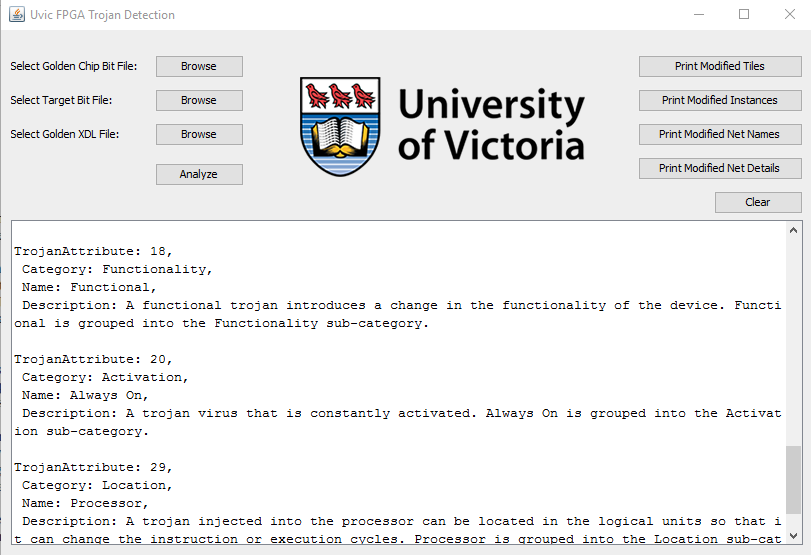
\includegraphics[width=1\linewidth]{Figures/backDoorResult}
\caption[Results of The Authentication Circuit Trojan Detection]{Results of The Authentication Circuit Trojan Detection}
\label{fig:backDoorResult}
\end{figure}

The system output the attributes:
\begin{itemize}
	\item Attribute 3: Fabrication
	\item Attribute 4: Testing
	\item Attribute 5: Assembly
	\item Attribute 6: System
	\item Attribute 7: RTL
	\item Attribute 12: Change in Functionailty
	\item Attribute 17: Combinational
	\item Attribute 18: Functional
	\item Attribute 20: Always On
	\item Attribute 24: Small
	\item Attribute 26: Augmented
	\item Attribute 27: Clustered
	\item Attribute 29: Processor
\end{itemize}
As expected the results state that the trojan was inserted in the Fabrication phase (3); it is the earliest stage in the 'insertion' phase produced indicating it as the source.
The effects of this modification propagate to the Testing (4) and Assembly (5) phases as expected.
The modifications reach both the System (6) and \acrfull{RTL} (7) abstraction levels.
Since the modifications were made using the schematic designer provided by \Xilinx which works in the \acrshort{RTL} level, these results are as expected.
The results indicate that the trojan Changes Functionality (12). 
This agrees with the modification to the values listed in Table~\ref{tbl:trojanOutputs}.
The trojan does not take affect over multiple clock cycles; this indicates it is composed of only Combinational (17) circuitry which is reflected in the results.
The trojan did not modify power levels or operation configurations, only design configurations.
This indicates that the trojan can be described as Functional (18), not Parametric (19); this agrees with the results.
Since the modification made a permanent alteration to the internal wiring of the circuit it can be said to be Always On (20).
The modified values for input $x=10$ or $x=11$ are always available and not activated.
This is consistent with the returned results.
The trojan changed only minor routing configurations in the circuit designs, this required the alteration of only a few tiles.
The new route required the activation of tiles which were not active in the \gls{golden} design; further, all of the modified tiles are nearby those in the \gls{golden} design. 
With these observations it can be said that this trojan exhibits Physical Layout attributes Small (24), Augmented (26) and Clustered (28). 
All of the expected Physical Layout attributes were correctly determined by the Scatter Score method of section~\ref{sec:scatterScore}.
Finally, all of the tiles modified by the trojan belong to major block type 0: Logic Type.
These tiles only affect the internal processing of the circuit.
No \acrshort{IOB}, Clock or \acrshort{BRAM} tiles were modified.
This is reflected by the fact that only Location attribute, Processor (29), was returned by the analysis.
The results observed by the experiment conformed with the experiments expectations demonstrating the accuracy of the method.
The entire analysis takes less than a minute to perform.
\subsection{AES-T100} \label{sec:aesT100}
In 2013 H. Salmani, M. Tehranipoor and R. Karri published a discussion on the design and development of \acrshort{FPGA} trojan benchmarks.
They collaboratively developed a series of verilog, VHDL and virtual machines that demonstrated effective creation of testable benchmarks.
They took the benchmarks they created and published them on a website they created called \textit{Trust-Hub}.
The benchmarks provided are organized by a taxonomy they proposed in~\cite{trustHubPaper}.
Their taxonomy is slightly different than the one used by the \NameNoPeriod which was proposed in~\cite{samerAttribute}, however the two are conceptually similar.
To demonstrate the efficacy of the \NameNoPeriod a benchmark named 'AES-T100' was chosen. 
The supporting documents describe this trojan as follows:
\begin{displaycquote}{trusthubWebsite}
	The Trojan leaks the secret key from a cryptographic chip running the AES algorithm through a covert channel. The channel adapts the concepts from spread spectrum communications (also known as Code-Division Multiple Access (CDMA)) to distribute the leakage of single bits over many clock cycles. The Trojan employs this method by using a pseudo-random number generator (PRNG) to create a CDMA code sequence, the PRNG initialized to a predefined value. The code sequence is then used to XOR modulate the secret information bits. The modulated sequence is forwarded to a leakage circuit (LC) to set up a covert CDMA channel in the power side-channel. The LC is realized by connecting eight identical flip-flop elements to the single output of the XOR gate to mimic a large capacitance.
\end{displaycquote}

From the description it is reasonable to expect certain results from the \Name.
The description states that the trojan 'leaks the secret key'.
From this we should expect our results to contain Effect attribute Information Leakage (13).
Information being leaked from a device will need a means to be transmitted to the attacker.
Location attribute \acrshort{IO} (31) may be observed.
It then states that it leaks 'single bits over many clock cycles'. 
This suggests that the trojan exhibits some form of Sequential Logic (16).
This may or may not require modification to clock tiles; Location attribute Clock Grid (33) may be observed. 
It then states that the PRNG is initialized to a predefined value; initialization requires the value be stored in memory. 
Location attribute Memory (30) should be expected.
The trojan then uses a 'power side-channel' as a communication channel.
This will require modification to power tiles; Location attribute Power Supply (32) should be expected.

The source code for the \gls{golden} and \gls{target} designs were downloaded from \textit{trust-hub.org} and synthesized on a Virtex-5 240T  (XC5VSX240T).
The analysis results were successfully found by the system as seen in Figure~\ref{fig:aesResult}.
\begin{figure}
\centering
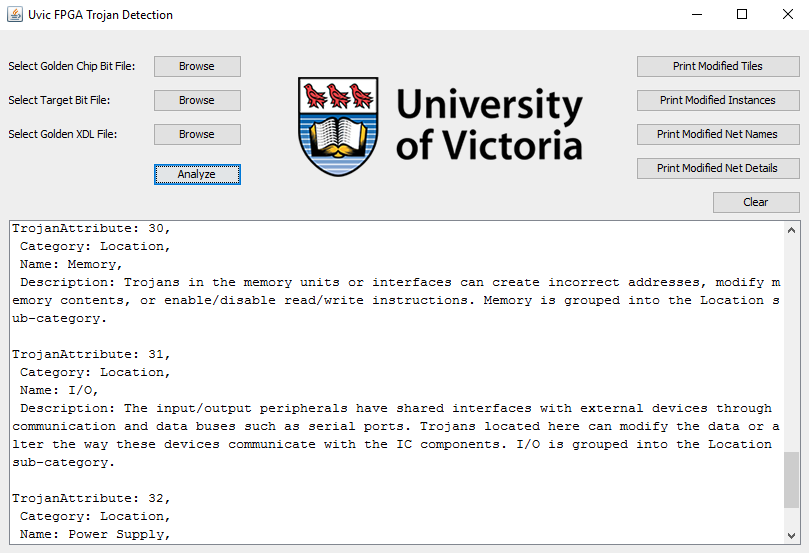
\includegraphics[width=1\linewidth]{Figures/aesResult}
\caption[Results of Analysis on the AES-T100 Benchmark]{Results of Analysis on the AES-T100 Benchmark}
\label{fig:aesResult}
\end{figure}

The \NameNoPeriod output the following attributes:
\begin{itemize}
	\item Attribute 3: Fabrication
	\item Attribute 4: Testing
	\item Attribute 5: Assembly
	\item Attribute 6: System
	\item Attribute 7: RTL
	\item Attribute 13: Information Leakage
	\item Attribute 16: Sequential
	\item Attribute 18: Functional
	\item Attribute 20: Always On
	\item Attribute 24: Large
	\item Attribute 26: Augmented
	\item Attribute 27: Distributed
	\item Attribute 29: Processor
	\item Attribute 30: Memory
	\item Attribute 31: \acrshort{IO}
	\item Attribute 32: Power Supply
	\item Attribute 33: Clock Grid
\end{itemize}

Again, it is assumed that this trojan was inserted during the fabrication phase; due to this the effects propagate to the Testing (4) and Assembly (5) phases.
Again, the trojan resides in the System (6) and \acrshort{RTL} (7) abstraction levels as was expected.
Attributes 13, 16, 30, 31, 32 and 33 appear in the analysis results as expected.
The Scatter Score method describes this trojan as Large, Augmented and Distributed. 
These results seem to correspond well with the description. 
The addition of the leakage circuit and the PRNG would be non-trivial addenda likely requiring the activation of considerable resources resulting in attribute Augmented (26).
Due to their complexity these added circuits will most likely need to be placed away from the \gls{golden} resources causing attribute Distributed (27).